\chapter{Hybrid evolutionary approach}
\label{chap:methodology}
%\minitoc

An evolutionary algorithm (GA) is a technique bio-inspired in the evolution of the spicies. It was proposed by John Holland, early in the 70's (Holland, 1975). This algorithm seeks to evolve a population of individuals that represent solutions to the problem through genetic operators such as crossover, mutations and selection. The population generated in each iteration is evaluated and then the individuals with a better fitness are chosen for the next generation with more chance.

\section{Hybrid evolutionary algorithm}

Hybrid evolutionary algorithms or hybrid genetic algorithms are very popular techniques that offer practical advantages to deal with complex and hardly optimization problems. Grosan (Grosan, 2007) presents a review of hybrid genetic architectures frecuently used. 

Hybridization can be performed using prior knowledge, heuristics, local search, and other techniques. We use it to carry out local search through rollout algorithm. Sometimes, a hybrid genetic algorithm which combine other technique to local search is known as memetic algorithm.

Generally, the purpose of hibridization is:

\begin{itemize}
 \item To improve the performance of the evolutionary algorithms.
 \item To improve quality of solutions obtained by evolutionary algorithm
 \item To incorporate evolutionary algorithm as part of a large system
\end{itemize}

Evolutionary algorithm behaviour is determined by the exploitation and exploration. In exploitation, local search is performed to improve solutions; in exploration, to avoid local optimum extending the search space, our implementation of memetic algorithm works to keep these relation throughout the run. Hence, in this application, the hybridazation not only improves the quality of the solutions obtained by evolutionary algorithm, but also  assembles as a framework for rollout algorithm in order to avoid local optimum.


\subsection{A basic genetic algorithm for vehicle routing problem with stochastic demands}

In figure \ref{fig:ga_basic} we show an example of a basic GA in general form. First, an initial population is selected and a fitness function is assessed for each individual in the population. In order to produce a new population for the next generation, crossover and mutation operators are applied to individuals, allowing those who have better fitness function to have more chances to reproduce themselves. In the selection stage, offspring's fitness is evaluated to choose the individuals which will integrate the new population; individuals with competitive fitness regarding population, have a higher probability to be selected. These steps are repeated until stopping criteriums are resolved.

\begin{figure}[!htbp]
  \begin{center}
   \includegraphics[width=0.6\textwidth]{Images/Chapter3/ga_basic.eps}
  \end{center}
    \caption{Basic genetic algorithm}\label{fig:ga_basic}
\end{figure}

\subsubsection*{Initialization}

We represent an individual in the population as a policy tour $\pi^\mathcal{C}$, whose fitness is the expected distance $\tilde{J}_{\pi^\mathcal{C}}$, computed using the algorithm $\Gamma$ \ref{algo:expecteddistance}.

The initial population $P_0$ with a fixed size $|P_0| = n$, is obtained using the cyclic heuristic in $O(n)$ time. It performs in this way to reduce the computational cost, since we can evaluate fitness to $P_0$ in $O(n)$ time when rollout is accomplished under some individual in the population.


\subsubsection*{Crossover}

The crossover operator $\circledast$ consists in the selection of two different individuals $I^{P_k}_i$ and $I^{P_k}_j$ with probability dependent on their fitness value, respectively; meanwhile, a random cut point $\rho \in [1,n]$ is uniformly selected in order to combine the parents' sequences to obtain a new sequence. Hence, a new individual raise to concatenate the subsequence $I^{P_k}_i[1..\rho]$ with the subsequence $I^{P_k}_j[\rho+1,..,n]$. 

A crossover operation can yield a new individual that represents an unfeasible policy. However, we implement this operator to run in time $O(n^2)$ and guarantee only feasible solutions as a result.


\subsubsection*{Mutation}

This operator performs three types of mutation with the same probability to produce and individual in the offspring: swap two elements of policy randomly selected, flip a random subsequence of policy or shift the policy a random number of times.

The mutation of an individual can happen with probability $Prob_m = 0.04$ in the experiments presented in this document, and compute in $O(1)$ time.


\subsubsection*{Selection of the new population}

New population originates as a result of crossover and mutation operators. Furthermore, the evolutionary algorithm also obtain individuals to the offspring performing the cyclic heuristic. Hence, those who have a better fitness can be chosen with more chance to integrate the new population.

In order to punish generation with fitness decrease and reward those who increase this value with respect to the previous generations, the size or number of individuals available to the next generation changes.

Let $\Delta^{P_k}_{E'}$ be the rate of fitness change in the generation $P_k$, i.e.

\begin{equation}\label{eq:improve_fitness}
 \Delta^{P_k}_{E'} = \frac{\bar{\Gamma}_{P_{k-1}} - \bar{\Gamma}_{P_k}}{\bar{\Gamma}_{P_{k-1}}} 
\end{equation}

where $\bar{\Gamma}_{P_k}$ is the best expected distance obtained by an individual in the generation $k$.

Then, the size of the next population $P_{k+1}$ is computed so that:

\begin{equation}\label{eq:population_size}
 ||P_{k+1}|| = \left \{ \begin{array}{ll}
  \lfloor  \min\{n(1+\alpha), ||P_{k}||(1+\alpha)\} \rfloor, & \text{if } \Delta^{P_k}_{E'} > 0\\
  \lceil \max\{n\alpha, ||P_{k}||\alpha\} \rceil, & \text{if } \Delta^{P_k}_{E'} < 0
  ||P_{k}||, \text{in other case.}
  \end{array} \right.
\end{equation}


where $\alpha$ is a tunable parameter which should be fixed in the range $(0,1]$ depending on computational resources. Consequently, this parameter reward a offspring that improve the quality of the solutions in comparison to their parents, increasing the population size at most an $\alpha$ times the size. Otherwise, when the quality of the solutions decreases with respect to the previous generation, the size of population is punished decreasing it at least a $\alpha$ factor of the population size. The figure \ref{fig:ga_basic_mvi_20r4_m} shows the results of basic genetic algorithm applied to one instance with $\alpha = 0.5$; below, the last chart on the right side of figure exhibits the size of population for each generation.

\begin{figure}[!htbp]
  \begin{center}
   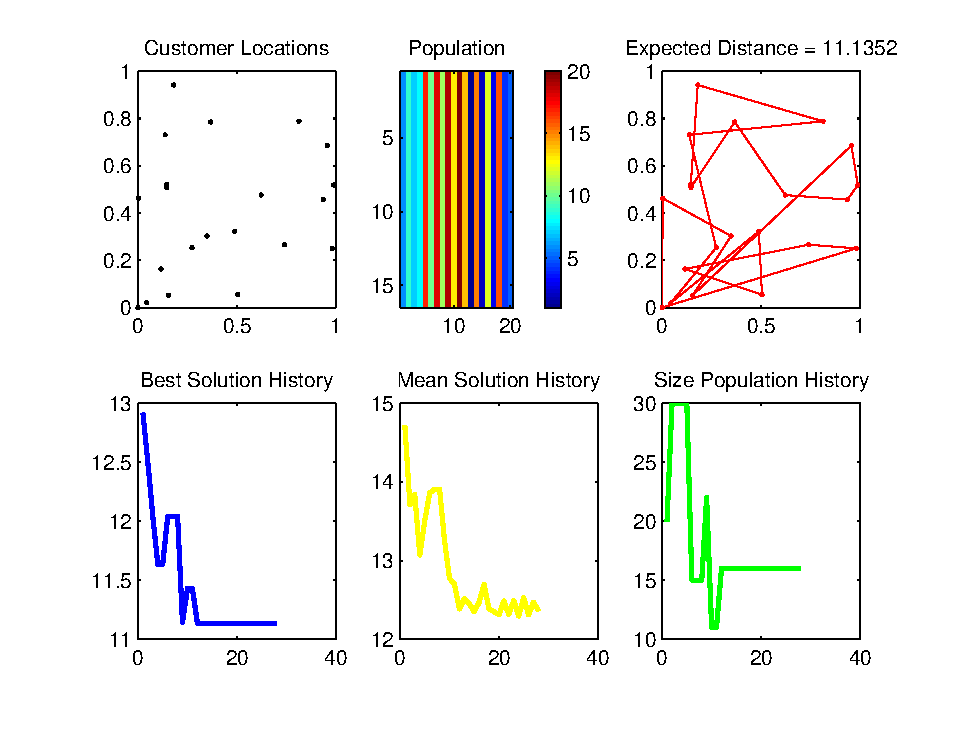
\includegraphics[width=0.9\textwidth]{Images/Chapter3/mvi_20r4_m_regular.eps}
  \end{center}
    \caption{Basic genetic algorithm applied to an instance of 20 customers. The second image in the first row ilustrate the last population and the next image shows the best solution found. }\label{fig:ga_basic_mvi_20r4_m}
\end{figure}

\subsubsection*{Stopping criterion}

Finally, the evolutionary algorithm runs until a fixed number or iterations $\kappa$ is reached. Nevertheless, it may stop once an $\mathbf{m}$ number of consecutive iterations without a significant change, i.e., $|\Delta^{P_k}_{E'}|\leq \varepsilon$ is accomplished. Both $\mathbf{m}$ and $\varepsilon$ are tunable parameters.

% \subsubsection{Crossover - EAX}

% Edge assembly crossover

% \subsubsection*{Mutation}

% Swap

\subsubsection*{Local search}


A classic genetic algorithm does not yield competitive results itself; due to basic GA, it does not exploit problem knowing to produce high quality solutions. In order to be effective, we combined local search methods. Local search can be incorporated in the initial population or among the offspring.

We applied the rollout algorithm as a local search method. The GA incorporates it in the initialization stage as in each iteration under the best policy obtained. Figure \ref{fig:memetic_mvi_20r4_m} shows the evolutionary algorithm with local search applied to the same instance used by the basic genetic algorithm above and showed in Figure \ref{fig:ga_basic_mvi_20r4_m}


\begin{figure}[!htbp]
  \begin{center}
   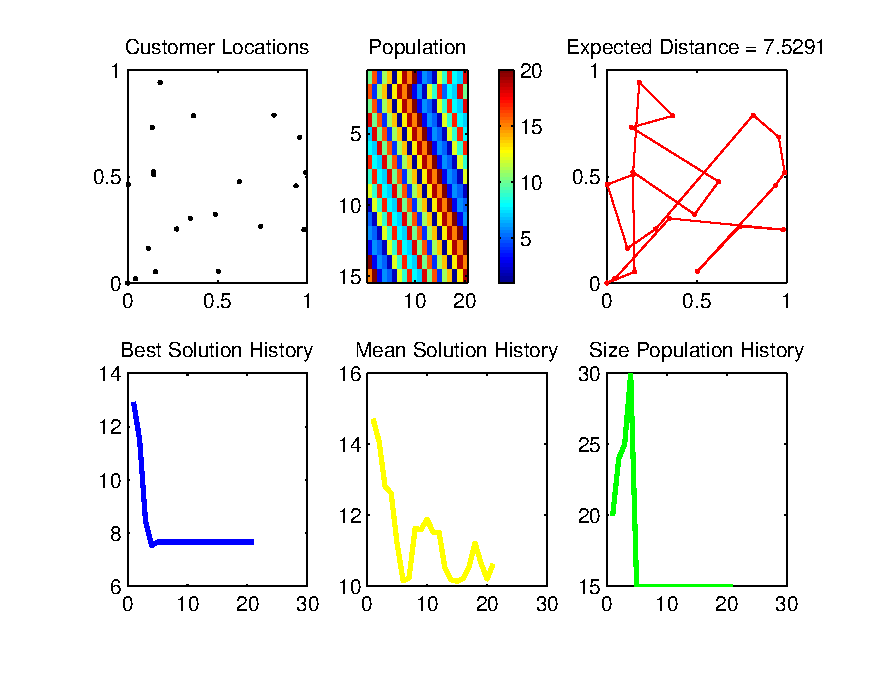
\includegraphics[width=0.9\textwidth]{Images/Chapter3/mvi_20r4_m_memetic.eps}
  \end{center}
    \caption{Memetic algorithm applied to an instance of 20 customers. The second image in the first row ilustrate the last population and the next image shows the best solution found.}\label{fig:memetic_mvi_20r4_m}
\end{figure}

\section{Summary}

In this chapter we presented a basic genetic algorithm for the vehicle routing problem with stochastic demands. In addition, we showed an hybrid approach, integrating the rollout algorithm as  a local search method in the evolutionary algorithm.